As stated by \citeonline{halliday2013fundamentals}, \emph{lenses} are objects consisting of a transparent material, with a certain refractive index, that are made of two spherical surfaces on which light propagates and suffers refraction. They are used in optical systems due to their capacity to create images as long as their refractive index is not equal to that of the medium. Yet, in agreement with \citeonline{halliday2013fundamentals}, some concepts related to lenses are important in our context and will be shown below. \autoref{fig:spherical_lens} illustrates an arbitrary spherical lens, with principal elements from geometric optics that relate to lenses and its consequent imaging properties.

\begin{figure}[htb]
	\centering
	\caption{\label{fig:spherical_lens} Arbitrary scheme of the optical properties of a spherical lens: radii of curvature ($r_{1}$, $r_{2}$), centers of curvature ($C_{1}$, $C_{2}$), focal points ($F_{1}$, $F_{2}$) and focal length ($f$).}
	\begin{center}
	    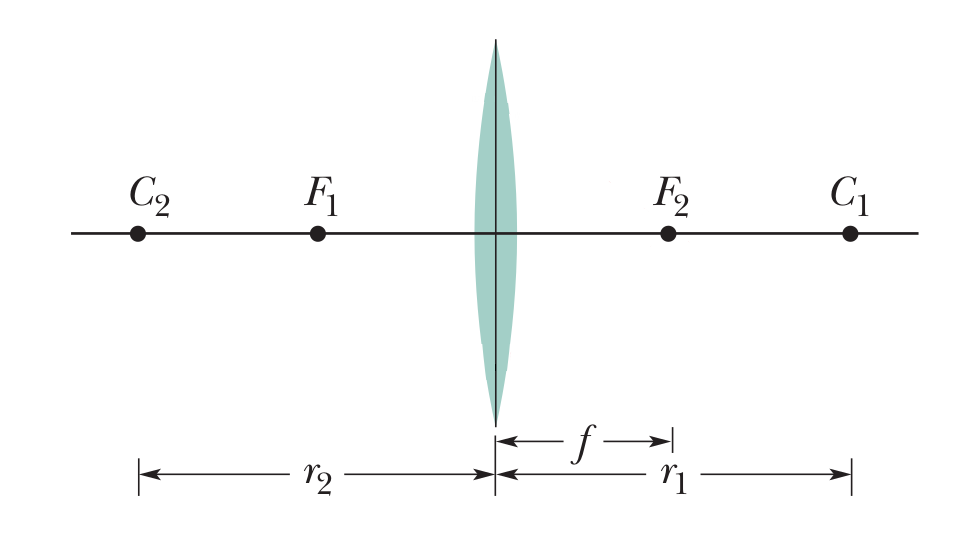
\includegraphics[scale=0.4]{images/fig4.png}
	\end{center}
	\centering
    \fadaptada{halliday2013fundamentals}
\end{figure}

Some properties of the spherical lenses directly influence the image formation process and, consequently, the resulting image quality. The \emph{numerical aperture} (NA), as reported by \citeonline{murphy2012fundamentals}, is a measurement in terms of angles that shows how much light the lenses can capture, and it is given by

\begin{equation}
    \label{eqn:numerical_aperture}
    NA = n \sin{\theta},
\end{equation}

\noindent where $\theta$ is the half angle of the cone of specimen light accepted by the objective lens and $n$ is the refractive index between the lens and the specimen. There are optical flaws in lenses that hinder a proper image formation. Those are named \emph{aberrations} \cite{lawlor2019introduction}, and the most relevant types in the scope of this project are the \emph{spherical aberrations}. According to \citeonline{murphy2012fundamentals}, the spherical aberrations occur when there is a difference in the focal point of incident parallel rays at central and peripheral locations of a spherical lens' surface, which yields a blurred image of either a point source of light or an extended object. It is possible to correct a spherical aberration by changing the shape of the refracting surface, i.e. changing the radius of curvature for the lenses in order to adjust the focal point to one particular distance \cite{smith1988optics}. The illustration in \autoref{fig:spherical_aberrations} represents the spherical aberration for a point source of light, where it is possible to see the difference between incident rays in the borders and in the inner regions of the lens. The resulting image is, in this case, a set of concentric circles around a point.

\begin{figure}[htb]
	\centering
	\caption{\label{fig:spherical_aberrations} Arbitrary example of the spherical aberration.}
	\begin{center}
	    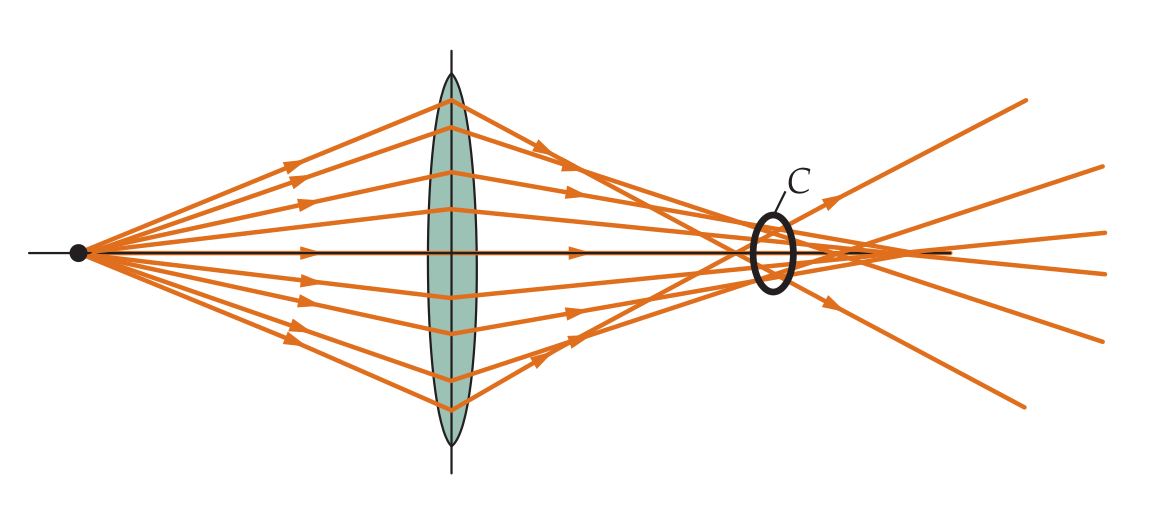
\includegraphics[scale=1.5]{images/spherical_aberration.png}
	\end{center}
	\centering
    \fdireta{tipler2008physics}
\end{figure}

\vspace{-1cm}